\section{Discussion}

\begin{figure}[!htbp]
\centering
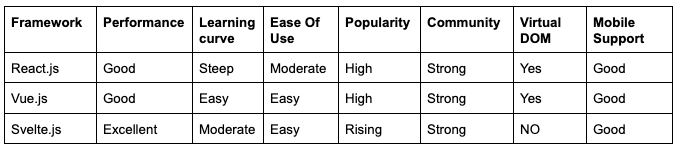
\includegraphics[width=\linewidth]{figs/compare.png}
\caption{compare}
\label{fig:compare}
\end{figure}

The table above presents a comparison chart for the frontend frameworks we have been working with. It assesses them on performance, learning curve, ease of use, size, popularity, community support, reusability, virtual DOM usage, and mobile support. Svelte.js is noted for its excellent performance and ease of use, while React.js and Vue.js are marked as good performers with strong community support and reusability. All three frameworks provide good mobile support, but only React.js and Vue.js utilize a virtual DOM, an approach that Svelte.js does not adopt.

\textbf{What Have We Learned?}

Throughout this project, our understanding of frontend frameworks has deepened significantly. We've learned the importance of choosing the right tool for the job: Vue for its simplicity and rapid prototyping, React for its robust ecosystem suitable for complex applications, and Svelte for its innovative approach and performance benefits. The exploration of these frameworks highlighted the trade-offs between ease of use, flexibility, and performance, an essential consideration for any web development project.

\textbf{What Would We Have Done Differently?}

In hindsight, a key area we would approach differently is the consideration of deployment aspects and how these frameworks integrate within a larger system with a custom-defined backend. We realize that the choice of frontend framework can significantly impact the overall architecture, scalability, and maintenance of web applications. Delving into how each framework interacts with different backend technologies would have provided a more holistic view of their capabilities in a real-world scenario. Additionally, exploring server-side rendering or static site generation options for each framework could have given us valuable insights into their performance and SEO advantages.

\textbf{Group Work and Work Distribution}

The group dynamics and work distribution were one of the strengths of this project. Each team member engaged early and showed enthusiasm, which fostered a collaborative and productive environment. We divided the work evenly, with each member focusing on a specific framework, allowing for a deep dive into each technology. This approach not only enhanced individual learning but also enriched our group discussions, as each member brought detailed insights and unique perspectives about their respective frameworks. Our regular weekly meetings and open communication ensured that the project progressed smoothly and cohesively.

\textbf{Future Work – Reflections on Further Development}

In our future work, we plan to delve deeper into the advanced capabilities of each framework and how they interact with different backend systems. We're particularly interested in how they fit into microservices architectures and serverless environments. We'll look at how they do in real deployment situations, focusing on load times, server-side rendering, and user experience. Alongside these technical evaluations, we also see the importance of user testing. By gathering feedback on how real users interact with the applications, we can understand the practical impact of each framework on user satisfaction and engagement. This feedback will be crucial in developing a set of best practices for building complex and user-friendly frontend systems.


The comparative analysis of ReactJS, Vue.js, and Svelte, as detailed in the article "Comparison and Analysis of Popular Frontend Frameworks and Libraries: An Evaluation of Parameters for Frontend Web Development" by Kaur and Tiwari, highlights the importance of examining how these frameworks approach UI design—a key aspect in frontend development (Kaur and Tiwari 5). React and Vue, while both being free, open-source, and performance-efficient, adopt distinct methodologies in their UI design processes. Svelte, on the other hand, also presents its unique approach to UI construction, which merits a closer examination.

Exploring the different resources available for Svelte, such as sveltematerialui.com by (Perrin), could provide valuable insights into its UI capabilities. This exploration would not only help in understanding Svelte’s design philosophy and practical application but also offer a perspective on how it compares with the UI design approaches of React and Vue. Such an analysis is crucial for developers to make informed decisions about which framework best suits their project's UI requirements.
